\documentclass[conference]{IEEEtran}
\IEEEoverridecommandlockouts
% The preceding line is only needed to identify funding in the first footnote. If that is unneeded, please comment it out.
\usepackage{cite}
\usepackage{amsmath,amssymb,amsfonts}
\usepackage{algorithmic}
\usepackage{graphicx}
\usepackage{textcomp}
\usepackage{xcolor}
\def\BibTeX{{\rm B\kern-.05em{\sc i\kern-.025em b}\kern-.08em
    T\kern-.1667em\lower.7ex\hbox{E}\kern-.125emX}}
\begin{document}

\title{Cost Effective Deployment of Hardware Accelerators Across Logic Simulator Modules}

\author{\IEEEauthorblockN{1\textsuperscript{st} Taten H. Knight}
\IEEEauthorblockA{\textit{College of Aviation, Science, and Technology} \\
\textit{Lewis University}\\
Romeoville, IL \\
tatenhknight@lewisu.edu}
}

\maketitle

\begin{abstract}
With the continuous growth of the the AI/ML sector and the need to increase the speed of learning and inference tasks, there has been increasing pressure to quickly produce, verify, and iterate on, System-on-Chip (SoC) configurations. A SoC configuration implies that the entire system ---CPU, gpu, memory, registers, etc. --- exist on a single board, versus the older paradigm of being made up of multiple physical chips. These systems are often deployed in safety-critical situations such as autonomous vehicle control and avionics, and the verified correctness of the system is quite literally life or death. They are also being deployed increasingly frequently in the mobile device space. The Apple M1 and subsequent "M" series processors, as well as Google's Pixel processor, are all SoC configurations. This configuration is often space saving and works well for small devices and it is also ultra-efficient. It reduces latency by decreasing the physical distance between components. This paper explores the history of PDES and distributed simulation algorithms, the evolution of the design of distributed discrete-event simulators, and the problems researchers and industry professionals face. There is an overview of the simulation architecture and an analysis of past and present algorithms and hardware advancements is performed. The paper wraps up with the proposal of a cost effective solution for simulator implementation, alongside explanation and justification of the proposal based on the relevant literature.
\end{abstract}

\begin{IEEEkeywords}
component, formatting, style, styling, insert
\end{IEEEkeywords}

\section{Introduction (1 Page)}
\subsection{Commercial Use}
The SoC is quickly becoming the gold standard for hardware as consumer tech-giants are attempting to outdo each other in terms of speed, efficiency, and price. At the same time, there has been a relatively recent revolution in the use of ML in consumer gadgets for increasing picture and video quality and verbal and written language processing. There has also been a shove for mass production of a fully autonomous vehicle, which requires custom silicon to be feasible at scale. The avionics industry were relatively early adopters of formal verification techniques for embedded systems; with the growth of the industry and newer, software dependent sub-systems, the task of writing test cases is unwieldy and unrealistic. The industry uses formal verification at the source code level for multiple requirements and sees significant savings for those requirements that are recurrent --- "a person-month per flight software release" \cite{b1}. Verification across a state-space that is not event-driven because the simulation is largely parallelizable, meaning that we are not constrained by maintaining sequential causal relationships across parallel state changes. A vehicle is a simple system, and although it does not lend itself well to parallelization, it can be adequately modeled with a reasonable amount of resources due to that low complexity.

\subsection{Academia}
The field of distributed systems and PDES (parallel discrete event simulation) has ballooned with the wide availability of cloud computing resources, the availability of super computing resources in academia via university sponsors and project funding, and overall out of necessity driven by industry growth. "PDES is concerned with the technologies associated with distributing the execution of a single run of a discrete event simulation program across multiple processors in a high performance computing system. Such platforms include shared-memory multiprocessors and message-based cluster computers. The central goal of PDES is typically to accelerate the execution of the simulation [...]. In contrast to parallel simulations where the processors executing the simulation reside within a cabinet inside a machine room, a distributed simulation may execute on a set of machines interconnected through a local area network, globally distributed computers communicating via the Internet, or predictive simulations embedded within a physical environment such as a sensor network monitoring traffic in a city" \cite{b2}. The problem of synchronization exists in both these fields, and with increases in network transfer speeds and bandwidth, PDES and distributed simulation studies continue to provide each other with new methodologies and approaches.

\section{The Problem (1 Page)}
The problem that we are presented with is the analysis of available technology (software, hardware, and algorithms), that can be implemented across the separate modules of the architecture shown in Fig.~\ref{arch} to increase overall efficiency, while remaining cost effective. 

\begin{figure}[htbp]
\centerline{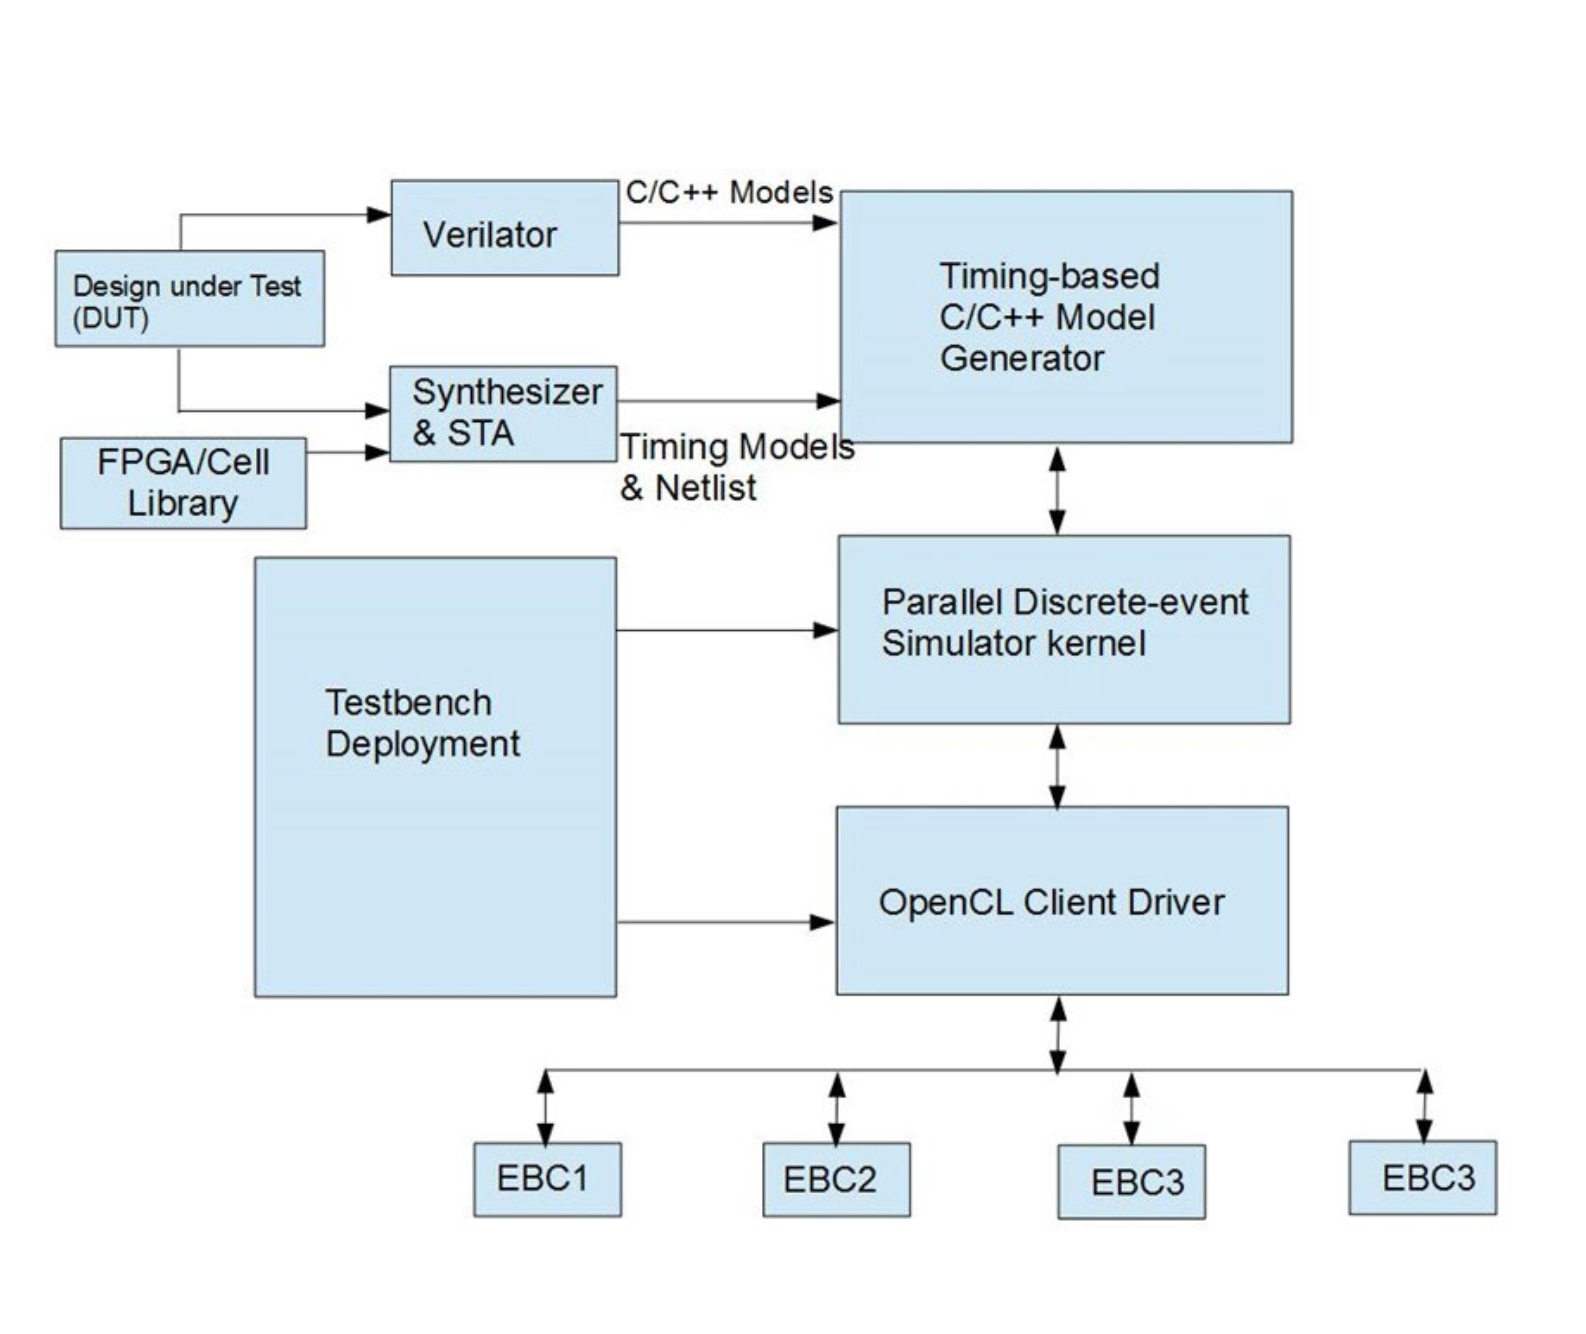
\includegraphics[width=\linewidth]{./images/architecture.png}}
\caption{Architecture of the Logic Simulator (EBC: Embedded Computing Module, STA: Static Timing Analyzer)}
\label{arch}
\end{figure}

Each module has unique characteristics to consider. There will be a basic overview of all of the modules in order to guarantee some level of contextual clarity for the discussion of a solution. 

\subsection{Design Under Test Module}
The aptly named design under test (DUT) module is the module that expresses the design in terms of some language (likely C or Verilog, considering the remainder of the architecture) \cite{b3} . This represents the current design that will be tested. 

\subsection{Verilator}
The DUT module feeds into two modules, one of which is the Verilator. Verilator is a free and open-source tool provided by Veripool that can be used to generate models based on the specified Verilog design. "Verilator is invoked with parameters similar to GCC or Synopsys's VCS. It "Verilates" the specified Verilog or SystemVerilog code by reading it, performing lint checks, and optionally inserting assertion checks and coverage-analysis points. It outputs single- or multi-threaded .cpp and .h files, the "Verilated" code"\footnote{https://www.veripool.org/verilator/}.

\subsection{FPGA/Cell Library}
"The FPGA generic architecture is composed of a matrix of configurable logic blocks (CLBs) [...] This matrix core is bordered by a ring of configurable input/output blocks (IOBs), whose number can reach 1000 user IOBs. Finally, all these resources communicate amongst themselves through a programmable interconnection network" \cite{b4}. A very high level FPGA diagram is shown in Fig.~\ref{fpga}.

\begin{figure}[htbp]
\centerline{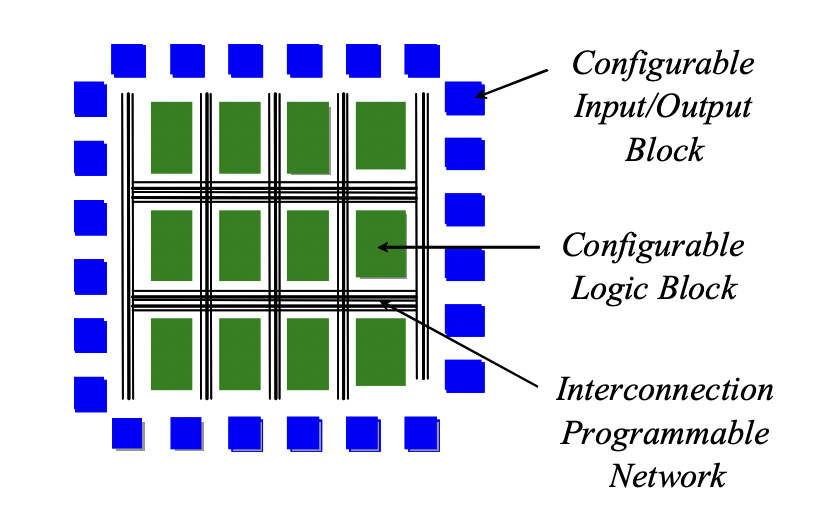
\includegraphics[width=\linewidth]{./images/fpga.png}}
\caption{Basic FPGA Diagram \cite{b4}}
\label{fpga}
\end{figure}

Each of the components shown is configurable, which has the potential to be overwhelming for a software engineer attempting to configure the chip without in depth knowledge of chip architecture. To mitigate this \cite{b4} manufacturers have provided cell libraries. A cell library is akin to a set of FPGA legos that can be used to design a chip.

\subsection{Synthesizer and STA Module}
The synthesizer and STA module takes both the DUT and FPGA configuration as inputs, and outputs the timing models for the software. This step is extremely important; when running a PDES, correct timing models are required to accurately determine synchronization of the discrete events. If the timings are inaccurate then the efficiency and speed of the simulation itself are mute.

\subsection{Timing Based C/C++ Model Generator}
The timing based C/C++ model generator combine the C/C++ models outputted by Verilator with the timing models from the synthesizer and STA module, and provide the final model that will be the input to the PDES simulator kernel.

\subsection{Testbench Deployment}
The testbench is both the physical and virtual environment within which the tests are ran. It includes the hardware of the deployment, and details such as the OS and other information that can affect the test runs.

\subsection{Parallel Discrete-event Simulator Kernel}
The PDES kernel is the core of the simulation. It distributes the event information to the OpenCL driver for processing, receives the information, and uses this information to update and distribute subsequent events. It also manages and provides final results to the testbench deployment.

\subsection{OpenCL Client Driver}
OpenCL drivers take events for calculation from the PDES kernel and distribute them to the appropriate embedded computing module, and direct the event simulation results back to the kernel.

\subsection{Embedded Computing Module}
Each embedded computing module (EBC) handles the processing of one discrete event or logical process (LP) at a time. These modules can be any type of chip that is appropriate to dealing with a certain event. With a local simulation each EBC is likely a CPU thread or core.

\section{Related Work (1 Page)}
\subsection{Chandy, Misra, and Bryant}
There is a myriad of work on methods for PDES acceleration. "The parallel and distributed simulation field began in the late 1970’s with seminal work by Chandy, Misra, and Bryant who defined the synchronization problem and a solution approach" \cite{b2}. When simulating discrete events of a DUT, it is essential that each event is simulated with all of the relevant information that would be relevant to that event in the real world, which means maintaining causality and continuity in the timing based model. The Chandy, Misra, and Bryant (CMB) algorithm is an elegant and simple solution to this problem. It guarantees that events are sent from LP to LP in timestamped order, and blocks the execution of an LP unless it is guaranteed that LP will not receive an earlier event. Fig.~\ref{cmb_deadlock} provides a visual explanation of the algorithm, as well as a visualization of one potential problem: deadlock.

\begin{figure}[htbp]
\centerline{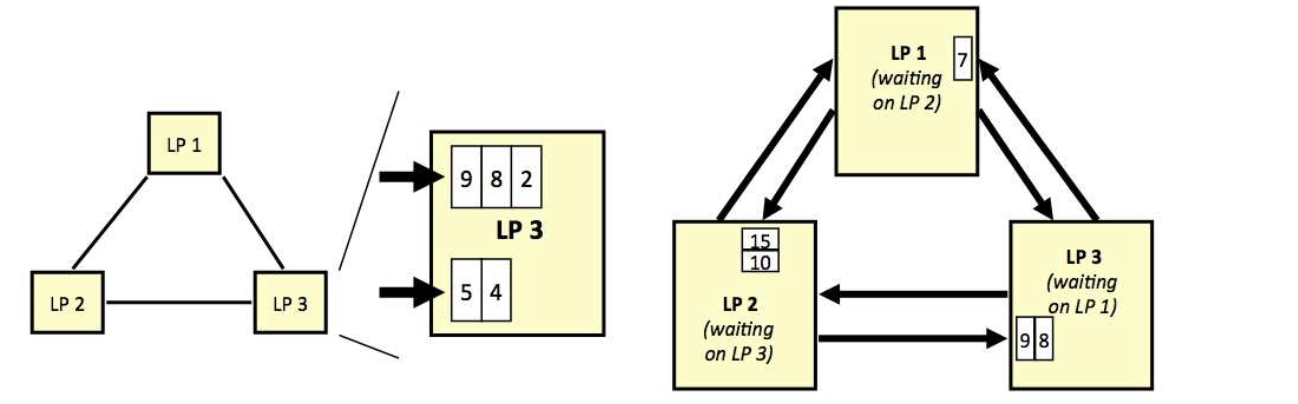
\includegraphics[width=\linewidth]{./images/cmb_deadlock.png}}
\caption{CMB Algorithm and Resultant Deadlock Case\cite{b2}}
\label{cmb_deadlock}
\end{figure}

CMB solves the deadlock by forcing each LP to send null messages with a carefully tuned lookahead value. "If an LP is currently at simulation time T, and its lookahead value is L, then any message later sent by the LP must have a timestamp of at least T+L" \cite{b2}. Fig.~\ref{lookahead} shows the benefits of having a lookahead value.

\begin{figure}[htbp]
\centerline{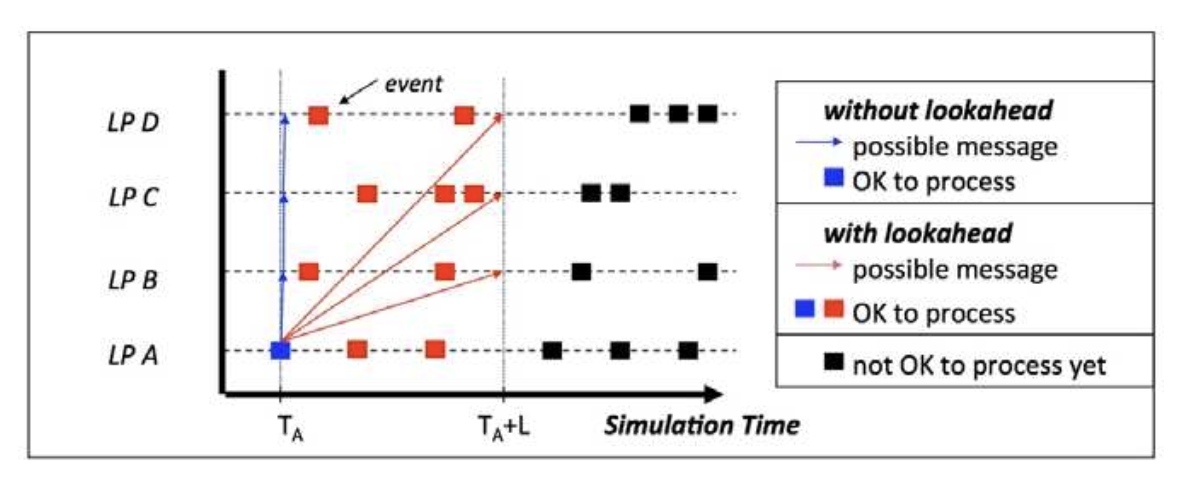
\includegraphics[width=\linewidth]{./images/lookahead.png}}
\caption{Benefits of lookahead value \cite{b2}}
\label{lookahead}
\end{figure}

A much larger number of events can be processed safely by having this value present. The lookahead value does need to be tuned well in order to avoid lookahead creep. Lookahead creep results in having a lookahead value that is potentially too small. If we have a value of .1 simulation seconds, and the next viable timestamp is 1 second above the current LP times, there will be ten LP messages sent that contain no event for processing, which consumes time.

\subsection{Second Generation Algorithms}
Second generation algorithms took advantage of the lessons learned from CMB. Two of these algorithms are Bounded Lag and YAWNS, both of which are synchronous algorithms. "meaning they utilize global synchronization points (barriers) as a fundamental element of the algorithm. These algorithms divide the computation into a sequence of cycles, or epochs. A global synchronization using a barrier primitive is used to separate the epochs. Each epoch involves (1) determining which events can be safely processed without risk of an LP later receiving a smaller timestamped event, (2) processing these safe events, possibly generating one or more new event messages, and (3) delivering these messages to their destination LPs. The computation repeatedly executes these epochs until the simulation has been completed" \cite{b2}. CMB and YAWNS are among the most popular algorithms to this day due to their simplicity and effectiveness, which is impressive considering they were developed in the late 70s and late 80s.

\subsection{Time Warp}
Time warp is the first optimistic synchronization algorithm. Optimistic algorithms allow errors to occur and establish methods for rolling back those errors when they are discovered. The Time Warp algorithm has a global control mechanism and a local control mechanism. When an error occurs (an event is processed out of error) there are two things that need to be reversed; sent messages triggered by the event and state changes made. There are three local control methods that handle state change rollback. \textit{Copy state saving} saves the state of the LP prior to processing each event. This consumes a large amount of memory as every state is temporarily saved for each LP. Next is \textit{incremental state saving} which saves the variable only before it is modified, allowing it to remain unsaved for an event if that event does not modify the state. This is much more efficient that copy state saving. Lastly there is \textit{reverse computation} which computes the reverse of a computation, for example if an event increments a variable, reverse computation decrements the variable. For some computations this reverse is not possible, and the program falls back to incremental state saving \cite{b2}. To undo sent messages, 'anti-messages' are sent, which signals the LP to reverse state changes and to send out another fleet of anti-messages that destroy those messages sent via the error. This can cause a cascade rollback wherein many anti-messages are sent and states reversed. This is the major downfall of an optimistic algorithm.
The global control mechanism established in \cite{b6} and improved upon in \cite{b7}.


\section{Potential Solution (1 Page)}
I propose a multi-level solution for the proposed research question that applies hardware acceleration and optimized algorithms at each possible module. This solution was developed by identifying the most obviously optimizable aspects of each module and finding well researched solutions. I also tried to keep the solutions realistic, avoiding a pure pay-for-performance approach in favor of a balanced solution.
\section{The Details (5 Pages)}
\subsection{FPGA/Cell Library}
A field programmable gate array (FPGA) 
\subsection{Design Under Test (DUT) Module}
\subsection{Verilator}
\subsection{Synthesizer and STA Module}
\subsection{Timing Based C/C++ Model Generator}
\subsection{Parallel Discrete-event Simulator Kernel}
\subsection{OpenCL Client Driver}
\subsection{Embedded Computing Module}
\section{Conclusion and Further Work (1 Page)}

\subsection{Maintaining the Integrity of the Specifications}

The IEEEtran class file is used to format your paper and style the text. All margins, 
column widths, line spaces, and text fonts are prescribed; please do not 
alter them. You may note peculiarities. For example, the head margin
measures proportionately more than is customary. This measurement 
and others are deliberate, using specifications that anticipate your paper 
as one part of the entire proceedings, and not as an independent document. 
Please do not revise any of the current designations.

\section{Prepare Your Paper Before Styling}
Before you begin to format your paper, first write and save the content as a 
separate text file. Complete all content and organizational editing before 
formatting. Please note sections \ref{AA}--\ref{SCM} below for more information on 
proofreading, spelling and grammar.

Keep your text and graphic files separate until after the text has been 
formatted and styled. Do not number text heads---{\LaTeX} will do that 
for you.

\subsection{Abbreviations and Acronyms}\label{AA}
Define abbreviations and acronyms the first time they are used in the text, 
even after they have been defined in the abstract. Abbreviations such as 
IEEE, SI, MKS, CGS, ac, dc, and rms do not have to be defined. Do not use 
abbreviations in the title or heads unless they are unavoidable.

\subsection{Units}
\begin{itemize}
\item Use either SI (MKS) or CGS as primary units. (SI units are encouraged.) English units may be used as secondary units (in parentheses). An exception would be the use of English units as identifiers in trade, such as ``3.5-inch disk drive''.
\item Avoid combining SI and CGS units, such as current in amperes and magnetic field in oersteds. This often leads to confusion because equations do not balance dimensionally. If you must use mixed units, clearly state the units for each quantity that you use in an equation.
\item Do not mix complete spellings and abbreviations of units: ``Wb/m\textsuperscript{2}'' or ``webers per square meter'', not ``webers/m\textsuperscript{2}''. Spell out units when they appear in text: ``. . . a few henries'', not ``. . . a few H''.
\item Use a zero before decimal points: ``0.25'', not ``.25''. Use ``cm\textsuperscript{3}'', not ``cc''.)
\end{itemize}

\subsection{Equations}
Number equations consecutively. To make your 
equations more compact, you may use the solidus (~/~), the exp function, or 
appropriate exponents. Italicize Roman symbols for quantities and variables, 
but not Greek symbols. Use a long dash rather than a hyphen for a minus 
sign. Punctuate equations with commas or periods when they are part of a 
sentence, as in:
\begin{equation}
a+b=\gamma\label{eq}
\end{equation}

Be sure that the 
symbols in your equation have been defined before or immediately following 
the equation. Use ``\eqref{eq}'', not ``Eq.~\eqref{eq}'' or ``equation \eqref{eq}'', except at 
the beginning of a sentence: ``Equation \eqref{eq} is . . .''

\subsection{\LaTeX-Specific Advice}

Please use ``soft'' (e.g., \verb|\eqref{Eq}|) cross references instead
of ``hard'' references (e.g., \verb|(1)|). That will make it possible
to combine sections, add equations, or change the order of figures or
citations without having to go through the file line by line.

Please don't use the \verb|{eqnarray}| equation environment. Use
\verb|{align}| or \verb|{IEEEeqnarray}| instead. The \verb|{eqnarray}|
environment leaves unsightly spaces around relation symbols.

Please note that the \verb|{subequations}| environment in {\LaTeX}
will increment the main equation counter even when there are no
equation numbers displayed. If you forget that, you might write an
article in which the equation numbers skip from (17) to (20), causing
the copy editors to wonder if you've discovered a new method of
counting.

{\BibTeX} does not work by magic. It doesn't get the bibliographic
data from thin air but from .bib files. If you use {\BibTeX} to produce a
bibliography you must send the .bib files. 

{\LaTeX} can't read your mind. If you assign the same label to a
subsubsection and a table, you might find that Table I has been cross
referenced as Table IV-B3. 

{\LaTeX} does not have precognitive abilities. If you put a
\verb|\label| command before the command that updates the counter it's
supposed to be using, the label will pick up the last counter to be
cross referenced instead. In particular, a \verb|\label| command
should not go before the caption of a figure or a table.

Do not use \verb|\nonumber| inside the \verb|{array}| environment. It
will not stop equation numbers inside \verb|{array}| (there won't be
any anyway) and it might stop a wanted equation number in the
surrounding equation.

\subsection{Some Common Mistakes}\label{SCM}
\begin{itemize}
\item The word ``data'' is plural, not singular.
\item The subscript for the permeability of vacuum $\mu_{0}$, and other common scientific constants, is zero with subscript formatting, not a lowercase letter ``o''.
\item In American English, commas, semicolons, periods, question and exclamation marks are located within quotation marks only when a complete thought or name is cited, such as a title or full quotation. When quotation marks are used, instead of a bold or italic typeface, to highlight a word or phrase, punctuation should appear outside of the quotation marks. A parenthetical phrase or statement at the end of a sentence is punctuated outside of the closing parenthesis (like this). (A parenthetical sentence is punctuated within the parentheses.)
\item A graph within a graph is an ``inset'', not an ``insert''. The word alternatively is preferred to the word ``alternately'' (unless you really mean something that alternates).
\item Do not use the word ``essentially'' to mean ``approximately'' or ``effectively''.
\item In your paper title, if the words ``that uses'' can accurately replace the word ``using'', capitalize the ``u''; if not, keep using lower-cased.
\item Be aware of the different meanings of the homophones ``affect'' and ``effect'', ``complement'' and ``compliment'', ``discreet'' and ``discrete'', ``principal'' and ``principle''.
\item Do not confuse ``imply'' and ``infer''.
\item The prefix ``non'' is not a word; it should be joined to the word it modifies, usually without a hyphen.
\item There is no period after the ``et'' in the Latin abbreviation ``et al.''.
\item The abbreviation ``i.e.'' means ``that is'', and the abbreviation ``e.g.'' means ``for example''.
\end{itemize}
An excellent style manual for science writers is \cite{b7}.

\subsection{Authors and Affiliations}
\textbf{The class file is designed for, but not limited to, six authors.} A 
minimum of one author is required for all conference articles. Author names 
should be listed starting from left to right and then moving down to the 
next line. This is the author sequence that will be used in future citations 
and by indexing services. Names should not be listed in columns nor group by 
affiliation. Please keep your affiliations as succinct as possible (for 
example, do not differentiate among departments of the same organization).

\subsection{Identify the Headings}
Headings, or heads, are organizational devices that guide the reader through 
your paper. There are two types: component heads and text heads.

Component heads identify the different components of your paper and are not 
topically subordinate to each other. Examples include Acknowledgments and 
References and, for these, the correct style to use is ``Heading 5''. Use 
``figure caption'' for your Figure captions, and ``table head'' for your 
table title. Run-in heads, such as ``Abstract'', will require you to apply a 
style (in this case, italic) in addition to the style provided by the drop 
down menu to differentiate the head from the text.

Text heads organize the topics on a relational, hierarchical basis. For 
example, the paper title is the primary text head because all subsequent 
material relates and elaborates on this one topic. If there are two or more 
sub-topics, the next level head (uppercase Roman numerals) should be used 
and, conversely, if there are not at least two sub-topics, then no subheads 
should be introduced.

\subsection{Figures and Tables}
\paragraph{Positioning Figures and Tables} Place figures and tables at the top and 
bottom of columns. Avoid placing them in the middle of columns. Large 
figures and tables may span across both columns. Figure captions should be 
below the figures; table heads should appear above the tables. Insert 
figures and tables after they are cited in the text. Use the abbreviation 
``Fig.~\ref{fig}'', even at the beginning of a sentence.

\begin{table}[htbp]
\caption{Table Type Styles}
\begin{center}
\begin{tabular}{|c|c|c|c|}
\hline
\textbf{Table}&\multicolumn{3}{|c|}{\textbf{Table Column Head}} \\
\cline{2-4} 
\textbf{Head} & \textbf{\textit{Table column subhead}}& \textbf{\textit{Subhead}}& \textbf{\textit{Subhead}} \\
\hline
copy& More table copy$^{\mathrm{a}}$& &  \\
\hline
\multicolumn{4}{l}{$^{\mathrm{a}}$Sample of a Table footnote.}
\end{tabular}
\label{tab1}
\end{center}
\end{table}

\begin{figure}[htbp]
\centerline{
\includegraphics{fig1.png}}
\caption{Example of a figure caption.}
\label{fig}
\end{figure}

Figure Labels: Use 8 point Times New Roman for Figure labels. Use words 
rather than symbols or abbreviations when writing Figure axis labels to 
avoid confusing the reader. As an example, write the quantity 
``Magnetization'', or ``Magnetization, M'', not just ``M''. If including 
units in the label, present them within parentheses. Do not label axes only 
with units. In the example, write ``Magnetization (A/m)'' or ``Magnetization 
\{A[m(1)]\}'', not just ``A/m''. Do not label axes with a ratio of 
quantities and units. For example, write ``Temperature (K)'', not 
``Temperature/K''.

\section*{Acknowledgment}

The preferred spelling of the word ``acknowledgment'' in America is without 
an ``e'' after the ``g''. Avoid the stilted expression ``one of us (R. B. 
G.) thanks $\ldots$''. Instead, try ``R. B. G. thanks$\ldots$''. Put sponsor 
acknowledgments in the unnumbered footnote on the first page.

\section*{References}

Please number citations consecutively within brackets \cite{b1}. The 
sentence punctuation follows the bracket \cite{b2}. Refer simply to the reference 
number, as in \cite{b3}---do not use ``Ref. \cite{b3}'' or ``reference \cite{b3}'' except at 
the beginning of a sentence: ``Reference \cite{b3} was the first $\ldots$''

Number footnotes separately in superscripts. Place the actual footnote at 
the bottom of the column in which it was cited. Do not put footnotes in the 
abstract or reference list. Use letters for table footnotes.

Unless there are six authors or more give all authors' names; do not use 
``et al.''. Papers that have not been published, even if they have been 
submitted for publication, should be cited as ``unpublished'' \cite{b4}. Papers 
that have been accepted for publication should be cited as ``in press'' \cite{b5}. 
Capitalize only the first word in a paper title, except for proper nouns and 
element symbols.

For papers published in translation journals, please give the English 
citation first, followed by the original foreign-language citation \cite{b6}.

\begin{thebibliography}{00}
\bibitem{b1} Y. Moy, E. Ledinot, H. Delseny, V. Wiels and B. Monate, "Testing or Formal Verification: DO-178C Alternatives and Industrial Experience," in IEEE Software, vol. 30, no. 03, pp. 50-57, 2013.
doi: 10.1109/MS.2013.43
\bibitem{b2} R. Fujimoto, "Parallel and Distributed Simulation", Proceedings of the 2015 Winter Simulation Conference, L. Yilmaz, W. K. V. Chan, I. Moon, T. M. K. Roeder, C. Macal, and M. D. Rossetti, eds
\bibitem{b3} R. C. Armstrong, R. J. Punnoose, M. H. Wong, J. R. Mayo, ``Survey of Existing Tools for Formal Verification'', in Sandia Report, 2014.
\bibitem{b4} E. Monmasson, M. Cirstea, ``FPGA Design Methodology for Industrial Control
Systems – a Review'', 
\bibitem{b5} R. Nane, V. Sima, C. Pilato, J. Choi, B.Fort, A. Canis, et al., ``A Survey and Evaluation of FPGA High-Level Synthesis Tools'' in IEEE Transactions on Computer-Aided Design of Integrated Circuits and Systems, vol. 35, no. 10, pp. 1591-1604, Oct. 2016, doi: 10.1109/TCAD.2015.2513673.
\bibitem{b6} B. Samadi, "Distributed Simulation, Algorithms and Performance Analysis", Computer Science
Department, University of California, Los Angeles, Los Angeles, California.
\bibitem{b7} F. Mattern, Efficient Algorithms for Distributed Snapshots and Global Virtual Time Approximation, Journal of Parallel and Distributed Computing, Volume 18, Issue 4, 1993, Pages 423-434, ISSN 0743-7315, https://doi.org 10.1006/jpdc.1993.1075.
\bibitem{b7} M. Young, The Technical Writer's Handbook. Mill Valley, CA: University Science, 1989.
\end{thebibliography}

\end{document}
